
    \begin{figure}[H]
      {
        \setlength{\tabcolsep}{3.0pt}
        \setlength\cmidrulewidth{\lightrulewidth} % Make cmidrule = 
        \begin{adjustbox}{width=0.5cm,center}
          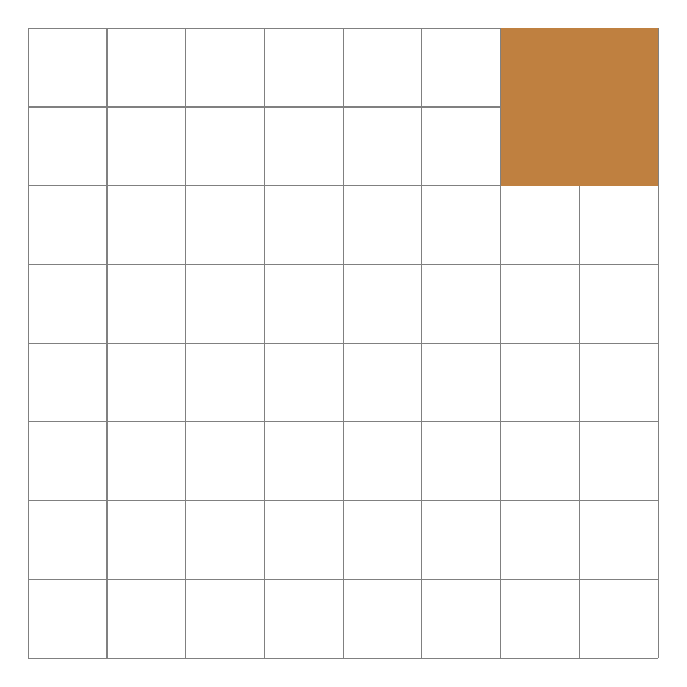
\begin{tikzpicture}
    
\def\BACKGROUNDONE{brown}
\def\BACKGROUNDTWO{lightblue}
\def\CHARCOLOR{lightgreen}
	\draw[step=1.0,gray,thin] (0,0) grid (8,8);
	\fill[\BACKGROUNDONE] (6,7) rectangle ++ (1,1);
	\fill[\BACKGROUNDONE] (7,7) rectangle ++ (1,1);
	\fill[\BACKGROUNDONE] (6,6) rectangle ++ (1,1);
	\fill[\BACKGROUNDONE] (7,6) rectangle ++ (1,1);

          \end{tikzpicture}
        \end{adjustbox}
      }\caption*{\$74}
    \end{figure}
    